\chapter{Introducción a la complejidad computacional}\label{anexoCC}
La teoría de complejidad computacional es la rama de las matemáticas y la ciencia de la computación que busca cuantificar los recursos necesarios para la resolución de problemas mediante algoritmos \cite{combarro-2023}. En este anexo se hará una pequeña introducción a los conceptos sobre complejidad computacional más importantes y necesarios para comprender el tipo de problemas tratados en el trabajo, aquellos conocidos como problemas $NP$-duros. Este capítulo estará basado principalmente en el libro sobre complejidad computacional de Sipser \cite{sipser-cc}. En primer lugar, se tratarán los conceptos básicos sobre autómatas, haciendo principal énfasis en las máquinas de Turing, esenciales para medir la computabilidad de un problema. A partir de estos conceptos se tratará la medición del tiempo de ejecución de los algoritmos y cómo se pueden clasificar los problemas a partir de este tiempo. Finalmente se mostrarán las clases de problemas más importantes, las clases $P$ y $NP$, además de las clases $NP$-completo y $NP$-duro.\\

\section{Autómatas, máquinas de Turing y tesis Church-Turing}
\begin{definition}
    Un autómata es un dispositivo teórico capaz de recibir y transmitir información. Dada una cadena de símbolos presentados a su entrada, produce una cadena de símbolos a la salida, en función de dichas entradas y los estados internos por los que transita la máquina.
\end{definition}
Dentro de los autómatas, podemos distinguir dos grupos fundamentales: los autómatas finitos, utilizados para el procesamiento de texto, en compiladores y en diseño de hardware; y los autómatas con pila, que son utilizados para definir lenguajes de programación y sistemas de inteligencia artificial. Para dar paso a las máquinas de Turing, que es lo que nos interesa, trataremos únicamente los autómatas finitos, para conocer más información sobre los autómatas con pila y las gramáticas sin contexto, se puede consultar el capítulo 2 de \cite{sipser-cc}. Podremos definir formalmente un autómata finito como:
\begin{definition}
    Un \textit{autómata finito} es una 5-tupla $(Q,\Sigma,\delta,q_0,F)$, donde
    \begin{enumerate}
        \item $Q$ es un conjunto finito de \textit{estados},
        \item $\Sigma$ es un conjunto finito denominado \textit{alfabeto},
        \item $\delta:Q\times \Sigma \rightarrow Q$ se denomina la \textit{función de transición} y define a que estado pasar dependiendo de un signo del alfabeto y el estado en el que se encuentra el autómata,
        \item $q_0$ es el \textit{estado inicial},
        \item $F\subseteq Q$ es el conjunto de \textit{estados aceptados} o \textit{estados finales}.
    \end{enumerate}
\end{definition}

Este tipo de autómatas reconoce un tipo de gramáticas denominados lenguajes regulares. Podemos ver un ejemplo del funcionamiento de un autómata finito mediante su diagrama de estados, un grafo dirigido cuyos ejes representan la función $\delta(q,a)$, donde $a$ representa el carácter a analizar (se muestra sobre los ejes del grafo) y $q$ el estado actual. Además, el estado final se ve representado como un círculo con un doble borde. En la Figura \ref{fig:automata-finito} podemos ver un diagrama de estados para un autómata que acepta cadenas que terminen en $0\,1$. Por ejemplo, rechazaría la cadena $1\,0\,1\,0$, ya que si seguimos las flechas, vemos que acabaría en el estado $q_1$, el cual no es un estado final. Sin embargo, la cadena $1\,0\,0\,1$ sí que sería aceptada.

\begin{figure}[b]
    \centering
    \begin{tikzpicture}[node distance=2cm, on grid, auto]
      \node[state, initial] (q0)   {$q_0$};
      \node[state]          (q1)   [right=of q0] {$q_1$};
      \node[state, accepting] (q2) [below=of q1] {$q_2$};
    
      \path[-to]
        (q0) edge [loop above] node {1} (q0)
             edge              node {0} (q1)
        (q1) edge [bend left, right] node {1} (q2)
             edge [loop above] node {0} (q1)
        (q2) edge [bend left, left] node {0} (q1)
             edge                   node {1} (q0);
    \end{tikzpicture}
    \caption{Autómata finito para el alfabeto $\Sigma = \{0,1\}$, que reconoce cualquier cadena que termina en $0\,1$.}
    \label{fig:automata-finito}
\end{figure}

Pasemos ahora a tratar un modelo más complicado, conocido como máquinas de Turing. Las máquinas de Turing funcionan de manera similar a un autómata finito pero tienen acceso a una memoria ilimitada y sin restricciones. Haciendo uso de estas características, las máquinas de Turing pueden verse como un modelo que representa un ordenador de propósito general, en particular, cualquier problema que pueda ser resuelto por una máquina de Turing puede ser resuelto por un ordenador. Es decir, si un problema no puede ser resuelto por una máquina de Turing, este problema será irresoluble. Una máquina de Turing puede definirse de manera formal de la siguiente manera.

\begin{definition}
    Una \textit{máquina de Turing} es una 7-tupla, $(Q,\Sigma,\Gamma,\delta,q_0,q_{acpt},q_{rechz})$, donde los conjuntos $Q,\Sigma,\Gamma$ son finitos y
    \begin{enumerate}
        \item $Q$ es el conjunto de estados,
        \item $\Sigma$ es el alfabeto de entrada que no contiene el símbolo en blanco $\sqcup$,
        \item $\Gamma$ es el alfabeto de la cinta, donde $\sqcup\in\Gamma$ y $\Sigma\subset \Gamma$,
        \item $\delta:Q\times \Gamma\rightarrow Q \times\Gamma\times\{L,R\}$ es la función de transición, es decir, a partir de un estado y un símbolo de entrada se pasa a un nuevo estado, escribiendo en la cinta un símbolo de $\Sigma$ y se mueve el cabezal a la izquierda ($L$) o a la derecha ($R$),
        \item $q_0\in Q$ es el estado inicial,
        \item $q_{acpt},q_{rechz}\in Q$ son el estado de aceptación y de rechazo respectivamente, y se cumple $q_{acpt}\neq q_{rechz}$.
    \end{enumerate}
\end{definition}

De manera más infomal, una máquina de Turing determinista es un dispositivo (teórico) formado por un cabezal de escritura/lectura y una cinta de longitud infinita. En una máquina de Turing, la cadena de entrada comienza escrita sobre la cinta. Al acabar de procesar la cadena, la salida se encontrará sobre la cinta. En cada paso del procesado, el cabezal lee el símbolo que se encuentra sobre la cinta, y, basándose en la función de transición $\delta$, pasará a otro estado, sobrescribiendo la posición de la cinta (o no) y moviendo el cabezal a la izquierda ($L$) o la derecha ($R$). El procesado finalizará si se alcanza un estado de parada, es decir, si alcanza un símbolo en blanco. Es posible que nunca se alcance un estado de parada, de hecho, el problema de conocer si una máquina de Turing va a terminar de procesar una entrada es un problema irresoluble. La prueba de esto puede ser encontrada en \cite{sipser-cc}.\\

Este modelo puede ser extendido a otros modelos de mayor complejidad. Por ejemplo, puede definirse un modelo que utiliza múltiples cintas o un modelo que permite la posibilidad de realizar múltiples acciones para la misma combinación de estado y símbolo en el que se encuentra la máquina, pudiendo estar en múltiples estados distintos al mismo tiempo. Denominamos a este último grupo máquinas de Turing no deterministas, y son muy importantes en la teoría de la complejidad computacional. Sin embargo, cualquier variación no es más potente que la máquina original, y cualquier problema que puede ser resuelto por una variación de una máquina de Turing básica puede resolverse también mediante una máquina de Turing determinista \cite{sipser-cc}.\\

Las máquinas de Turing son de gran interés debido a su estrecha relación con el concepto de algoritmo. Aunque un algoritmo puede entenderse informalmente como un conjunto de instrucciones que permiten resolver una tarea, esta definición carece de formalidad. Para formalizar la noción de algoritmo, surge la tesis de Church-Turing, la cual establece una conexión entre la definición informal de algoritmo y la definición formal basada en las máquinas de Turing. Según esta tesis, toda función que pueda ser calculada mediante un procedimiento efectivo también puede ser computada por una máquina de Turing.

\section{Medición del tiempo computacional}
Según la tesis de Church-Turing, para ver si un problema puede ser resuelto de manera algorítmica, se puede usar cualquier modelo equivalente a una máquina de Turing determinista. Sin embargo, si tratamos los recursos y el tiempo que se necesita para realizar este cálculo, no todos los modelos son equivalentes. Para calcular el tiempo computacional, se deberá fijar como base uno de los modelos. En nuestro caso (es el estándar para toda la teoría de la computación), se fijará como modelo una máquina de Turing determinista.\\

El número de pasos que necesite un algoritmo puede variar por múltiples motivos, sin embargo, para evitar estos problemas se definirá el tiempo de ejecución o complejidad temporal de una máquina de Turing determinista como una función de la longitud de la entrada.

\begin{definition}
    Sea $M$ una máquina de Turing determinista que se para para cualquier entrada. El \textit{tiempo de ejecución} o \textit{complejidad temporal} de $M$ es la función $f:\mathbb{N}\rightarrow\mathbb{N}$, donde $f(n)$ es el número máximo de pasos que $M$ utiliza para analizar cualquier entrada de longitud $n$. Si $f(n)$ es el tiempo de ejecución de $M$, se dice que $M$ se ejecuta en tiempo $f(n)$.
\end{definition}

Debido a que utilizar el tiempo exacto para medir el número de pasos de un algoritmo es una labor complicada, se utiliza el denominado análisis asintótico del crecimiento de las funciones. Para ello, utilizamos la notación de la cota superior asintótica o notación O Grande, representada con el carácter $\mathcal{O}$. 

\begin{definition}
    Sean $f$ y $g$ funciones tales que $f,g:\mathbb{N}\rightarrow\mathbb{R}^+$. Se dice que $f(n)=\mathcal{O}(g(n))$ si existen $c,n_0\in \mathbb{N}$ tales que para cada $n\geq n_0$,
    $$f(n)\leq cg(n).$$
    Es decir, que la función $g(n)$ es una cota superior asintótica (se ignoran los factores constantes) de la función $f(n)$.
\end{definition}

De esta manera, se puede medir el tiempo de ejecución de un algoritmo (o de una máquina de Turing determinista) como su comportamiento asintótico, sin tener que mirar los valores específicos que toma la función.

\section{P y NP}
Una vez definidos los conceptos anteriores, es posible realizar la clasificación de los distintos problemas computacionales en distintos grupos dependiendo de su complejidad (la complejidad intrínseca del problema, no de los algoritmos existentes para resolverlos). En este ámbito, se puede considerar un problema como un conjunto infinito de instancias para los cuales se espera una salida. Podemos representar un problema como una función que produce una salida a partir de una entrada, es decir, podremos representar un problema mediante una máquina de Turing. De esta manera, utilizando las ideas de las secciones anteriores, se puede estudiar qué problemas pueden ser resueltos mediante máquinas de Turing y cuanto tiempo será necesario \cite{combarro-2023}.\\

En la complejidad computacional, el tipo más sencillo de problemas son los denominados problemas de decisión. La salida de este tipo de problemas es un valor booleano (verdadero o falso), y algún ejemplo importante de este tipo de problema puede ser el problema de determinar si un grafo tiene un camino hamiltoniano o el problema de la parada de una máquina de Turing.

\begin{definition}
    Se dice que una máquina de Turing $M$ es \textit{decisora} para un problema de decisión si para cualquier entrada del problema se produce una decisión final. En este caso también se dice que la máquina de Turing $M$ \textit{resuelve el problema}.
\end{definition}

Utilizando esta definición se tiene que existen decisores para el problema del camino hamiltoniano, pero no para el problema de la parada. Por consiguiente, el primer problema se denomina \textit{decidible}, mientras el segundo es \textit{indecidible}.\\

Con esta idea, conociendo qué es un problema decidible, se pueden definir clases de complejidad dependiendo del tiempo utilizado por la máquina de Turing que resuelve el problema. En primer lugar, podemos definir la clase de complejidad $P$.

\begin{definition}
    Se dice que un problema $A$ \textit{pertenece a la clase de complejidad} $P$ o $A\in P$ si existe una máquina de Turing $M$ tal que su tiempo de ejecución sea de orden polinómico. Esto es, dado $f(n)$ el tiempo de ejecución de $M$, entonces $f(n)=\mathcal{O}(n^a),\;a\in\mathbb{N}$.
\end{definition}

Se debe tener en cuenta que para ver que un problema pertenece a $P$, sirve con encontrar un decisor de orden polinómico para ese problema. No obstante, para demostrar que un problema no pertenece a $P$, será necesario probar que no existe ninguna máquina de Turing que se ejecute en tiempo $\mathcal{O}(n^a)$. Una característica interesante de la clase $P$, es que para otras variaciones de máquinas de Turing (deterministas), cualquier problema que sea decidible en tiempo polinómico por estas, también lo va a ser por una máquina de Turing básica (consultar \cite{sipser-cc} para la prueba).\\

La otra clase principal de complejidad computacional es la clase $NP$. La clase $NP$ está formada por aquellos problemas que pueden ser verificados en tiempo polinómico.

\begin{definition}
    Dado un problema $A$, se dice que $A$ tiene un \textit{verificador en tiempo polinómico} si existe una máquina de Turing $M$ que se ejecuta en tiempo polinómico y un polinomio $q$ tales que:
    \begin{itemize}
        \item Si $x$ es una instancia del problema $A$ de tamaño $n$ tal que la respuesta sea verdadero, entonces existe una cadena binaria $y$ de longitud máxima $q(n)$ tal que la decisión de $M$ para $(x,y)$ sea verdadero. La cadena $y$ se denomina \textit{certificado}.
        \item Si $x$ es una instancia del problema $A$ de tamaño $n$ tal que la respuesta sea falso, entonces para cualquier cadena binaria $y$ de longitud máxima $q(n)$, la decisión de $M$ para $(x,y)$ es falso. 
    \end{itemize}
\end{definition}

Esto nos indica que dada una instancia del problema cuya solución sea verdadera, podemos encontrar un certificado (de longitud polinómica) tal que sea aceptado por la máquina de Turing $M$. Sin embargo, para cualquier instancia cuya solución sea falsa, no existe tal certificado. Si se elimina la condición de la longitud polinómica de la cadena, se tendrá la definición de un verificador. Otra manera de definir el conjunto $NP$ es la siguiente. La prueba de este resultado puede encontrarse en \cite{sipser-cc}.

\begin{theorem}
    Un problema $A$ \textit{pertenece a la clase de complejidad} $NP$ o $A\in NP$ si y solo si existe una máquina de Turing \textbf{no determinista} $M$ tal que su tiempo de ejecución sea de orden polinómico.
\end{theorem}

Algún ejemplo de problema que pertenece a $NP$ es el problema de los caminos hamiltonianos de un grafo. El certificado en este caso es un camino hamiltoniano (tiene longitud polinómica). Si tenemos un camino, ver que es hamiltoniano es polinómicamente verificable. Sin embargo, si el grafo no tiene caminos hamiltonianos, no existe ningún certificado. Es trivial ver que cualquier problema que pertenezca a $P$ pertenece a $NP$, ya que podemos usar el decisor del problema como verificador. Por consiguiente, $P\subset NP$. Podría parecer que probar que los conjuntos $P$ y $NP$ son distintos es sencillo, sin embargo, esto no es así.

\section{Reducciones, completitud y dureza}
Aunque la decisión sobre si $P=NP$ es compleja, a lo largo de los años se han realizado distintas investigaciones que indican que existen ciertos problemas en $NP$ cuya complejidad individual está relacionada con la de toda la clase. Es decir, si se descubriese algún algoritmo polinómico para alguno de estos problemas, todos los problemas de $NP$ serían resueltos en tiempo polinómico. Este tipo de problemas se denominan $NP$-completos. Sin embargo, para poder definir este tipo de problemas será necesario tratar el concepto de reducción.

\begin{definition}
    Dado $\Sigma^*=\{w_0w_1\cdots w_i\cdots/w_i\in\Sigma\}$ el conjunto de cadenas de longitud variable formado por elementos del alfabeto $\Sigma$, una función $f:\Sigma^*\rightarrow\Sigma^*$ se denomina \textit{función computable} si para cada entrada $w$, una máquina de Turing $M$ se para con únicamente $f(w)$ en su cinta. En concreto, si $M$ es una máquina de Turing de tiempo polinómico, se dice que $f$ es una \textit{función computable en tiempo polinómico.}
\end{definition}

\begin{definition}
    Un problema $A$ es \textit{reducible} a otro problema $B$, representado como $A\leq_m B$, si existe una función computable $f:\Sigma^*\rightarrow\Sigma^*$, donde para cada $w$,
    $$w\in A \iff f(w)\in B.$$
    La función $f$ se denomina \textit{reducción} de $A$ a $B$. Si la función $f$ es computable en tiempo polinómico, se dice que el problema $A$ es \textit{reducible en tiempo polinómico} a $B$ y se representa como $A\leq_pB$. En este caso la función $f$ se denomina \textit{reducción en tiempo polinómico} de $A$ a $B$.
\end{definition}

Las reducciones conservan las características computacionales de los problemas. Por ejemplo, se tiene el siguiente teorema.

\begin{theorem}
    Sean $B$ un problema decidible y $A$ otro problema tal que $A\leq_mB$. Entonces, $A$ es decidible.
\end{theorem}

En particular, si tenemos una reducción en tiempo polinómico tendremos un resultado más interesante.

\begin{theorem}\label{th:ainpreduc}
    Si $A\leq_pB$ y $B\in P$, entonces $A\in P$.
    \begin{proof}
        Dado $M$ el algoritmo (o máquina de Turing) en tiempo polinómico que decide $B$ y sea $f$ una reducción en tiempo polinómico de $A$ a $B$. Se puede describir el siguiente algoritmo en tiempo polinómico $N$ que decida $A$ de la siguiente manera:
        \begin{align*}
            N = & \text{``Para la entrada } w:\\
            & 1.\;\; \text{Computar } f(w).\\
            & 2.\;\; \text{Ejecutar } M \text{ para la entrada } f(w) \text{ y utilizar como salida la salida de } M. \text{''}
        \end{align*}
        Como $f$ es una reducción de $A$ a $B$, se tiene que $w\in A$ si $f(w)\in B$. Por consiguiente, $M$ acepta $f(w)$ siempre que $w\in A$, es decir, $N$ es decidible. Además, $N$ se ejecuta en tiempo polinómico, ya que los dos pasos descritos se ejecutan en tiempo polinómico.
    \end{proof} 
\end{theorem}

Un corolario de este resultado es el siguiente.
\begin{corollary}
    Si dado un problema $A\notin P$, entonces si $A\leq_pB$ se tiene que $B\notin P$.
\end{corollary}

Volviendo a la idea que comenzó este capítulo, ahora sí podemos definir los problemas $NP$-completos.

\begin{definition}
    Un problema $B$ es $NP$\textit{-completo} si satisface 2 condiciones:
    \begin{enumerate}
        \item $B\in NP$,
        \item cada problema $A\in NP$ es reducible en tiempo polinómico a $B$.
    \end{enumerate}    
\end{definition}

Conociendo su definición, ahora tiene sentido la afirmación con la que comenzaba el capítulo. Esta afirmación puede escribirse de la siguiente manera.

\begin{theorem}
    Si $B$ es $NP$-completo y $B\in P$ entonces $P=NP$.
    \begin{proof}
        Como $B$ es $NP$-completo, cualquier problema $A\in NP$ es reducible en tiempo polinómico a $B$. Ahora, utilizando el Teorema \ref{th:ainpreduc}, se tendrá que todo problema $A$ pertenecerá a $P$. Por consiguiente, $NP\subset P$, y $P=NP$.
    \end{proof}
\end{theorem}

Otro subconjunto de los problemas de $NP$ interesante es el conocido como problemas $NP$-duros.
\begin{definition}
    Un problema $B$ es $NP$\textit{-duro} si cada problema $A\in NP$ es reducible en tiempo polinómico a $B$.
\end{definition}

Como podemos observar esta clase de problemas es similar a los problemas $NP$-completos, pero no tienen la restricción de pertenecer a la clase $NP$. Es decir, se tendrá la siguiente relación: $NP\text{-completo}\subset NP\text{-duro}$. La eliminación de esta restricción implica que exista algún problema $NP$-duro que no sea verificable en tiempo polinómico o que incluso no sea verificable ni decidible. Algún problema que pertenece a esta clase es por ejemplo el problema del agente viajero o TSP, el cual es una reducción en tiempo polinómico de los problemas de rutas que se tratan en este trabajo. Para comprender mejor esta relación, la Figura \ref{fig:venncc} contiene un diagrama de Venn que explica la relación que existe entre los conjuntos de problemas tratados para dos casos, el primero en el que $P\neq NP$ y para un segundo caso donde $P=NP=NP\text{-completo}$.
\begin{figure}[H]
    \centering
    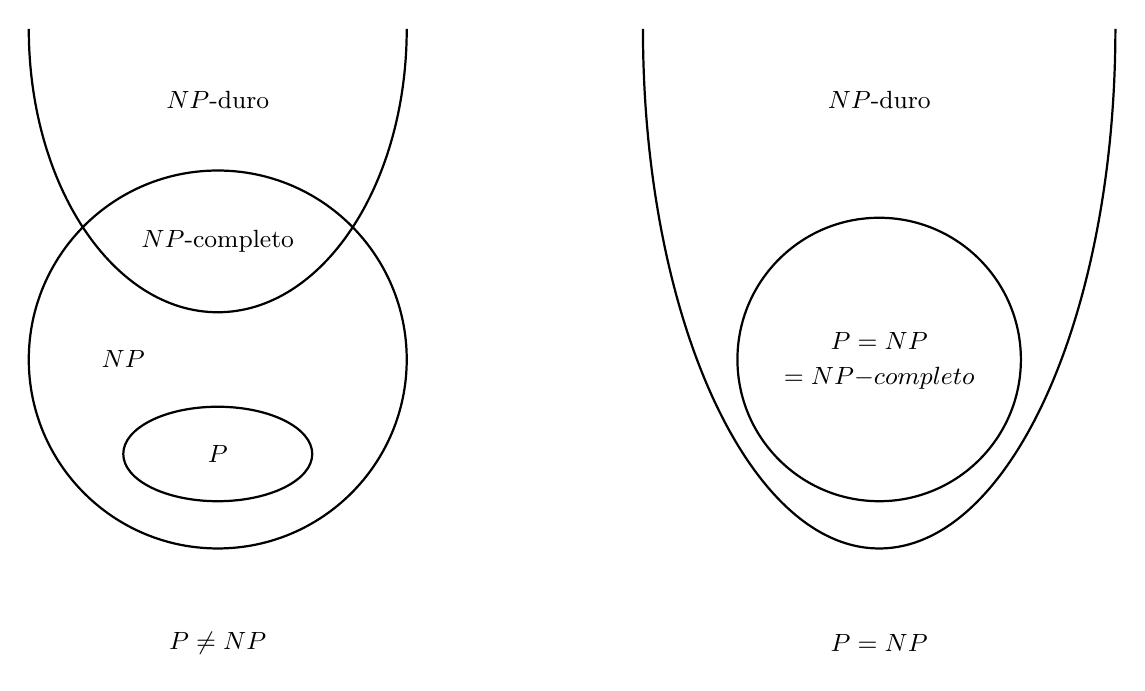
\begin{tikzpicture}[scale=1.2, every node/.style={font=\small}]        
        \begin{scope}
            \draw[thick] (0,0) circle (2);
            \node at (-1,0) {$NP$};
            \draw[thick] (0,-1) ellipse (1 and 0.5);
            \node at (0,-1) {$P$};
            \draw[thick] (-2,3.5) arc[start angle=180, end angle=360, x radius=2, y radius=3];
            \node at (0,1.25) {$NP$-completo};
            \node at (0,2.75) {$NP$-duro};
            \node at (0,-3) {$P\neq NP$};
        \end{scope}
        \begin{scope}[xshift=7 cm]
            \draw[thick] (0,0) circle (1.5);
            \node at (0,0.2) {$P=NP$};
            \node at (0,-0.2) {$= NP\text{-completo}$};
            \draw[thick] (-2.5,3.5) arc[start angle=180, end angle=360, x radius=2.5, y radius=5.5];
            \node at (0,2.75) {$NP$-duro};
            \node at (0,-3) {$P= NP$};
        \end{scope}
    \end{tikzpicture}
    \caption{Diagrama de Venn que representa la relación entre las clases de complejidad tratadas en el capítulo. A la izquierda se muestra el caso en el que $P\neq NP$ a la derecha, el caso en el que $P=NP$.}
    \label{fig:venncc}
\end{figure}